\documentclass{article}
\usepackage{listings}
\usepackage{amsmath}
\usepackage{fullpage}
\usepackage{tabularx}
\usepackage{graphicx}
\usepackage{tikz}
\usetikzlibrary{shapes.geometric, arrows}
\usepackage{cite}
\usepackage{hyperref}
\usepackage{float}
\begin{document}
\lstset{language=python, tabsize=4}
\title{Node mapping}
\maketitle

\begin{abstract}
	We present node mapping, a machine learning technique created for numerical 
	link attribute prediction tasks in a graph.
	Using this technique, the estimator builds a neural net model, learns to 
	represent every node in the graph as a node vector of real numbers(mapping 
	nodes to vectors), and learns to predict the target link attribute using 
	these node vectors.
	The main idea is to extract information about nodes from links and use this 
	information to predict unknown link attributes.
	We demonstrate the usage and high accuracy of this technique in a movie 
	rating prediction task.
\end{abstract}

\section{Introduction}

\subsection{Background}
Both academia and industry have seen pervasive adoption of deep learning 
techniques powered by artificial neural network models since early 2010s, when 
they began to outperform other machine learning techniques in various 
application domains (e.g., speech recognition \cite{hannun2014deep}, image 
recognition \cite{simonyan2014very}, and natural language processing 
\cite{yao2013recurrent}).
These neural net models can not only achieve higher prediction accuracy than 
traditional models, but also require much less domain knowledge and engineering.
Moreover, neural net models have participated in more general artificial 
intelligence design by complementing search techniques, demonstrated by
Google AlphaGo AI when it defeated go champion Lee Sedol in 2016 
\cite{silver2016mastering}.
Specifically, in a game like go with simple rules but too many possible 
configurations to explore, neural net models achieve good results with 
reasonable computing resources, which are easily exhausted by algorithms solely 
powered by search.

\subsection{Motivation}
As neural nets have demonstrated their power in many domains, we naturally 
wonder if we can apply them in prediction tasks in graph mining domain, and 
what kind of techniques are helpful in using their power.
There are existing techniques with promising results already.
Two earlier attempts were graph neural nets and relational neural 
nets \cite{scarselli2009graph}, where neural nets are incorporated into a 
traditional iterative graph information propagation approach.
A later attempt was deep walk \cite{perozzi2014deepwalk}, where a graph is 
reduced to a natural language corpus so that existing neural net models 
designed for natural language processing can handle the graph.
These attempts all have an essential idea of applying neural net in 
graphs: converting graph to numerical variables.
This idea is essential in other application domains as well, because neural 
nets cannot directly handle non-numerical variables.
We initiated our research hoping to create a simpler, more direct technique 
that can take advantage of rich structured graph information.
We are particularly interested in application scenarios like making 
recommendations for social network users based on user activities including 
messaging friends, commenting articles, and rating movies.

\subsection{Goal}
We want to create a technique to predict link attributes in a graph using a 
neural net model.
The graph can have any topology and its links can have a numerical attribute.
The estimator should learn to represent the graph in a meaningful way and to 
learn to predict the target link attribute using the representation it learns.

\section{Observations and approach}

\subsection{Entities, representations and relations in different domains}
In order to find out how a neural net can predict link attributes, we first 
review how it handles entities in different domains.
\autoref{tab:domains} provides a summary of various types of entities, their 
numerical representations and inter-entity relations in different domains.
\begin{table}[h]
	\centering
	\begin{tabularx}{\textwidth}{ |c|c|c|X| } \hline
		domain & entity & representation & relations to other entities \\ \hline
		image recognition & image & 2D light intensity array & NA \\ \hline 
		speech recognition & utterance/spectrogram & 2D sound intensity array & 
		NA \\ \hline
		natural language & word & word vector & relations to other words \\ 
		\hline
		graph & movie & node vector & directed by director, etc \\ \hline
		graph & user & node vector & rate movies, etc \\ \hline
	\end{tabularx}
	\caption{A summary of various types of entities, their numerical
		representations and inter-entity relations in different domains:
		Images and utterances can be directly represented by 2D numerical 
		arrays, but have no strong relations to other images or utterances. 
		words and various types of nodes in graphs can represented by vectors 
		(1D numerical arrays) and have strong relations to other words and 
		nodes.}
	\label{tab:domains}
\end{table} 
Notice that the representations for all the entities are numerical arrays, 
because neural nets rely on neurons' activations and communications, which 
are both numerical.

\subsection{Mapping word to vectors}
Words can be mapped to vectors by word2vec technique 
\cite{mikolov2013efficient}.
In word2vec, a neural net learns to map every word in a vocabulary to a vector 
without any domain knowledge.
\autoref{tab:word} shows a mapping table that maps each word ID to the word 
vector.
\begin{table}[h]
	\centering
	\begin{tabularx}{0.5\textwidth}{|X|X|} \hline
		word ID & word vector \\ \hline
		1 & [2.3, 564, -9.5 ... 3] \\ \hline
		2 & [76, -342.2, 0.3 ... 4.2] \\ \hline
		3 & [-345, -834, 0.3 ... 34] \\ \hline
		... & ... \\ \hline
		n & $ [x_1, x_2, x_3 ... x_d] $ \\ \hline
	\end{tabularx}
	\caption{Word to vector mapping table for a vocabulary of size n with word 
	vectors of size d:
	Each word has its ID and its characters don't matter (possibly Chinese or 
	Hindi).
	Each vector is randomly initialized before learning and then gradually 
	updated by the neural net during learning.}
	\label{tab:word}
\end{table}
In a corpus, every word is described/defined only by related words in its 
context, although relations between the words are implicit. 
Nonetheless, the neural net can learn from word co-occurrences (i.e., 
relations) and map words to vectors accordingly such that the relations between 
words are preserved in the vector space \cite{mikolov2013distributed}.

\subsection{Mapping node to vectors}
If we compare language data and graph data, we can see they have many 
similarities, shown in \autoref{tab:wordVSnode}.
\begin{table}[h]
	\centering
	\begin{tabularx}{\textwidth}{ |X|X|X| } \hline
		aspect  & natural language processing & graph mining \\ \hline
		dataset & corpus & graph \\ \hline
		basic entities & words & nodes \\ \hline
		entity collection & vocabulary & node set \\ \hline
		relations & co-occurrences (implicit) & links (explicit) \\ \hline
		representation & word vectors & node vectors \\ \hline
	\end{tabularx}
	\caption{A comparison of language data and graph data from 
		several aspects: these similarities suggest a neural net might be able 
		to map nodes to node vectors just like mapping words to word vectors.}
	\label{tab:wordVSnode}
\end{table}
Apparently, mapping node to vectors should be more direct than mapping word to 
vectors, because the relations between nodes are explicit(i.e., link and link 
attributes), while relations between words are implicit(i.e., word 
co-occurrences).
In a social network example, the rating a movie received from a user explicitly 
tells us how much the user likes that movie; the number of messages a user 
sends to another user explicitly tells us how close they are connected.
In a language corpus example, the co-occurrences of words [the, quick, brown, 
fox, jumps, over] implicitly suggest these words may be related but do not tell 
us what their relations are.
This suggests that a neural net should be able to learn node mapping supervised 
by the link attributes in a more direct way than it learns word mapping 
supervised by word co-occurrences.

\section{Application scenario}

\subsection{Scenario: recommendations in a social network}
We first demonstrate an application scenario node mapping technique is designed 
to handle: making recommendations to users in social network.
This is a simplified social network where users can send messages to other 
users and give ratings to movies.
The service provider is interested in recommending friends and movies for each 
user, solely based on how much he communicates to other users and how much 
he likes different movies.
Formally, the graph is:
\begin{itemize}
	\item a node set consisting of 2 types of nodes: users and movies
	\item a link set consisting of 2 types of links: user-user links with 
	numerical attribute called messages indicating the amount of messages the 
	user has sent to the other user(e.g., total number of messages, words 
	or characters in the past 12 months),
	and user-movie links with numerical attribute called rating indicating the 
	rating the user has given to the movie(e.g., a number in range(0, 5))
\end{itemize}
If we can build an estimator to predict the messages attribute of user-user 
links (or the rating attribute of user-movie links), we can know how much a 
user would like each of the users (movies) he has not connected to (rated) and 
recommend those he would like the most to him.
Formally, the prediction task is:
\begin{itemize}
	\item input: X = (node1, node2)
	\item output: Y = link(node1, node2).attribute
\end{itemize}
In the following, we will demonstrate how to use this technique in rating 
prediction.
We also expect it (with moderate modifications) to work for messages 
prediction, but we currently haven't verified that experimentally.

\subsection{Dataset: MovieLens 100K}
We evaluate the prediction accuracy of this technique using MovieLens 100k 
dataset \cite{harper2015movielens} 
\footnote{http://grouplens.org/datasets/movielens/100k/}. This dataset has the 
following specs:
\begin{itemize}
	\item number of users: 1000
	\item number of movies: 1700
	\item number of ratings: 100,000
\end{itemize}
and a few samples are shown in \autoref{tab:rating}.
\begin{table}[h]
	\centering
	\begin{tabularx}{0.5\textwidth}{ |X|X|X| }  \hline
		user ID & movie ID & rating \\ \hline
		0 & 355 & 4 \\ \hline
		0 & 876 & 3 \\ \hline
		0 & 232 & 5 \\ \hline
		1 & 324 & 2 \\ \hline
		... & ... & ... \\ \hline
	\end{tabularx}
	\caption{The Movie Lens dataset: Every link has 1 numerical attribute - 
	rating.}
	\label{tab:rating}
\end{table}
The dataset is split into 3 sets as in normal machine learning experiments:
\begin{itemize}
	\item training set: 70\%
	\item validation set: 10\%
	\item test set: 20\%
\end{itemize}

\subsection{Prediction task: rating prediction}
The model will need to predict the ratings in the testing set: given any (user, 
movie) pair, it needs to predict the rating given to the movie by the user:
\begin{itemize}
	\item input: X = (user, movie)
	\item output: Y = rating(user, movie)
\end{itemize}

\section{Implementation}

\subsection{Conceptual model: fully-connected neural net}
The estimator includes a fully-connected neural net model, shown in 
\autoref{fig:conceptural}.
\begin{figure}[h]
	\centering
	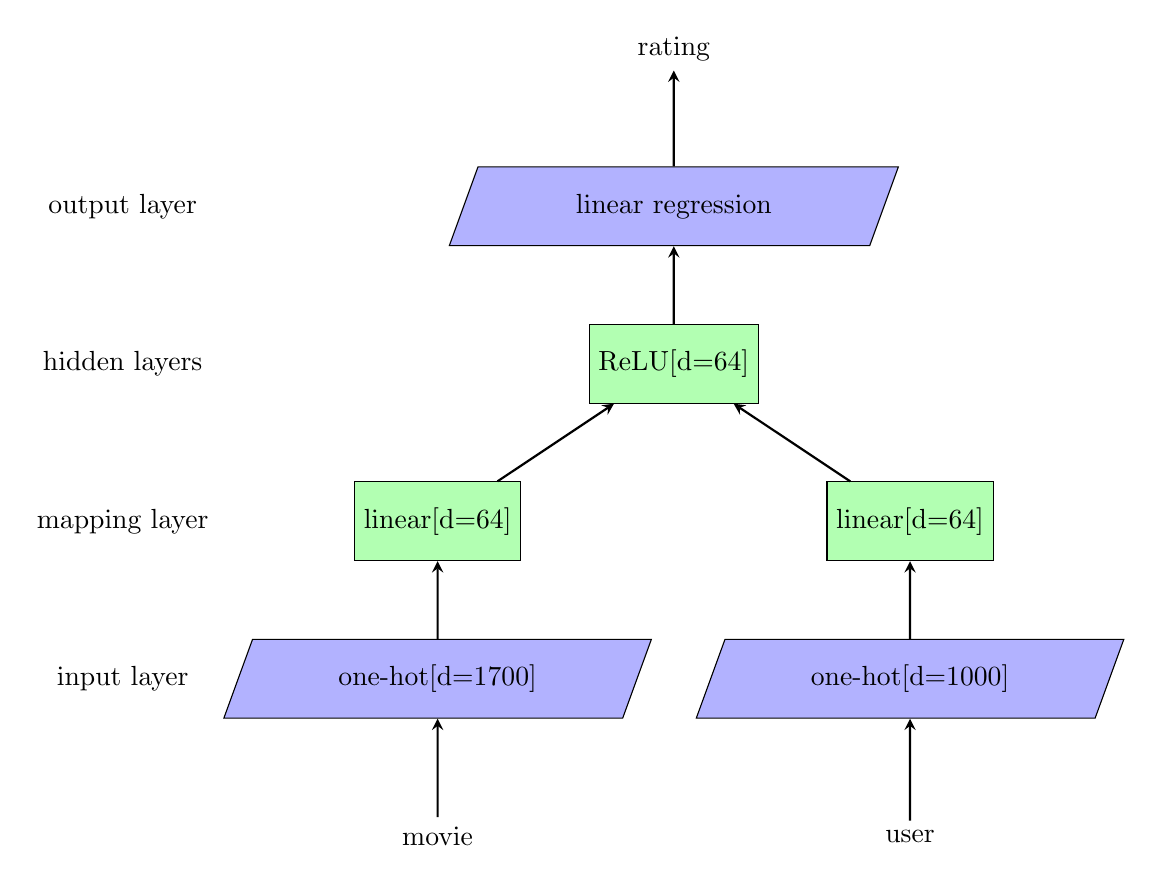
\begin{tikzpicture}[node distance=2cm]
	\tikzstyle{io} = [trapezium, trapezium left angle=70, trapezium right 
	angle=110, minimum width=1cm, minimum height=1cm, text centered, 
	draw=black, fill=blue!30]
	\tikzstyle{process} = [rectangle, minimum width=1cm, minimum height=1cm, 
	text centered, draw=black, fill=green!30]
	\tikzstyle{arrow} = [thick,->,>=stealth]
	\node (linearRegression) [io] {linear regression};
	\node (relu3) [process, below of=linearRegression] {ReLU[d=64]};
	\node (linear2) [process, below of=relu3, xshift=-3cm] {linear[d=64]};
	\node (linear1) [process, below of=relu3, xshift=3cm] {linear[d=64]};
	\node (oneHot2) [io, below of=linear1] {one-hot[d=1000]};
	\node (oneHot1) [io, below of=linear2] {one-hot[d=1700]};
	\node (rating) [above of=linearRegression] {rating};
	\node (output) [left of=linearRegression, xshift=-5cm] {output layer};
	\node (hidden1) [below of=output] {hidden layers};
	\node (mapping) [below of=hidden1] {mapping layer};
	\node (input) [below of=mapping] {input layer};
	\node (movie) [below of=oneHot1] {movie};
	\node (user) [below of=oneHot2] {user};
	\draw [arrow] (movie) -- (oneHot1);
	\draw [arrow] (user) -- (oneHot2);
	\draw [arrow] (oneHot2) -- (linear1);
	\draw [arrow] (oneHot1) -- (linear2);
	\draw [arrow] (linear1) -- (relu3);
	\draw [arrow] (linear2) -- (relu3);
	\draw [arrow] (relu3) -- (linearRegression);
	\draw [arrow] (linearRegression) -- (rating);
	\end{tikzpicture}
	\caption{The conceptual fully-connected neural net model for a dataset
		with 1700 movies and 1000 users:
		The d in the bracket refers to dimension, the layer's size (number of 
		units in the layer).
		We keep all layers the same size for simplicity, although layers of 
		different sizes may produce better results.
		The text before the bracket refers to the activation function of the 
		units in the layer(except for one-hot, which refers to the activations 
		in the input layer).
		Only layers and their connections are shown, while the units in each 
		layer and their connections are not shown.}
	\label{fig:conceptural}
\end{figure}
The model contains following layers:
\begin{itemize}
	\item an input layer with one-hot activations: it has 1 channel for movies 
	and 1 channel for users;
	this layer is directly activated by the testing program (e.g., to feed the 
	1200th movie, the testing program sets 1 at the 1200th unit and 0 at other 	
	units in the movie channel)
	\item a mapping layer with linear units: it has 2 channels to map each 
	movie (and each user) to a vector;
	the activations of these 2 channels form the 2 node vectors(i.e., the movie 
	vector and the user vector);
	it is the most critical layer as it gradually learns to map every node to 
	the correct vector during training;
	\item several hidden layers(only 1 layer is shown in the figure) of 
	ReLU(rectified linear unites):
	they have non-linear activation functions to give the model sufficient 
	complexity; 
	they learn to process node vectors and produce more abstract 
	rating-relevant information;
	\item an output layer with a linear regression unit: it learns to predict 
	the rating based on processed information;
\end{itemize}

\subsection{Actual model: fully connected neural net and mapping tables}
In practice, it's not efficient or scalable to use a one-hot input layer, 
especially if the graph contains many nodes.
\autoref{fig:actural} shows the actual model used in action with 2 
modifications from the conceptual model:
\begin{itemize}
	\item The input layer becomes a 2 mapping tables: 1 for movie nodes and 1 
	for user nodes;
	their inputs are node IDs and their outputs are node vectors, just like the 
	word to vector mapping table shown in \autoref{tab:word}
	\item The mapping layer becomes a 2-channel input layer: it is directly 
	activated by the outputs of the mapping tables
\end{itemize}
\begin{figure}[h]
	\centering
	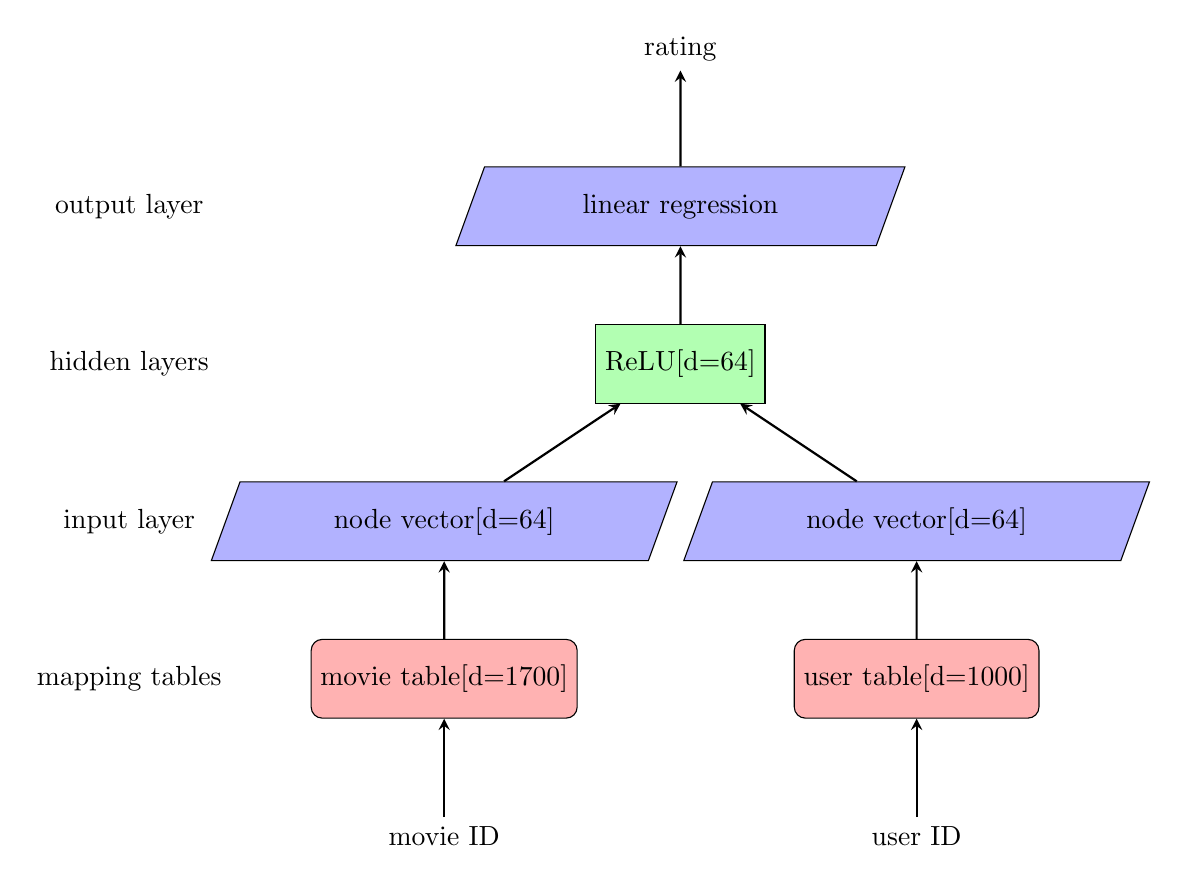
\begin{tikzpicture}[node distance=2cm]
	\tikzstyle{io} = [trapezium, trapezium left angle=70, trapezium right 
	angle=110, minimum width=1cm, minimum height=1cm, text centered, 
	draw=black, fill=blue!30]
	\tikzstyle{startstop} = [rectangle, rounded corners, minimum width=1cm, 
	minimum height=1cm, text centered, draw=black, fill=red!30]
	\tikzstyle{process} = [rectangle, minimum width=1cm, minimum height=1cm, 
	text centered, draw=black, fill=green!30]
	\tikzstyle{arrow} = [thick,->,>=stealth]
	\node (linearRegression) [io] {linear regression};
	\node (relu3) [process, below of=linearRegression] {ReLU[d=64]};
	\node (linear2) [io, below of=relu3, xshift=-3cm] {node vector[d=64]};
	\node (linear1) [io, below of=relu3, xshift=3cm] {node vector[d=64]};
	\node (oneHot2) [startstop, below of=linear1] {user table[d=1000]};
	\node (oneHot1) [startstop, below of=linear2] {movie table[d=1700]};
	\node (rating) [above of=linearRegression] {rating};
	\node (output) [left of=linearRegression, xshift=-5cm] {output layer};
	\node (hidden1) [below of=output] {hidden layers};
	\node (input) [below of=hidden1] {input layer};
	\node (mapping) [below of=input] {mapping tables};
	\node (movie) [below of=oneHot1] {movie ID};
	\node (user) [below of=oneHot2] {user ID};
	\draw [arrow] (movie) -- (oneHot1);
	\draw [arrow] (user) -- (oneHot2);
	\draw [arrow] (oneHot2) -- (linear1);
	\draw [arrow] (oneHot1) -- (linear2);
	\draw [arrow] (linear1) -- (relu3);
	\draw [arrow] (linear2) -- (relu3);
	\draw [arrow] (relu3) -- (linearRegression);
	\draw [arrow] (linearRegression) -- (rating);
	\end{tikzpicture}
	\caption{The actual implementation with 2 modifications:
		We factor the node to vector mapping process out of the neural net into 
		2 node to vector mapping tables.
		We feed every node (a movie or user) to the estimator by feeding the 
		node ID.
		During learning, the estimator updates the vectors in the tables the 
		same way it updates weights in the conceptual model.}
	\label{fig:actural}
\end{figure}
We have an open source implementation available for interested readers and we 
are open to collaborations \footnote{https://github.com/yuchenhou/elephant}.
We build an estimator with the above neural net model and popular learning 
techniques for neural net including SGD(stochastic gradient descent) and its 
variant Adagrad(advanced gradient descent), mini-batch, and dropout.
The code is in Python and the main machine learning package is TensorFlow 
\cite{tensorflow2015-whitepaper}.

\section{Experiments}

\subsection{Learning process}
The estimator learns for several epochs.
During each epoch, it updates its model by fitting the training set, and 
then evaluates the learning progress by performing prediction using the 
validation set.
It logs the average training error and average validation error for each epoch 
and stops learning when the validation error starts increasing to reduce 
over-fitting.
After learning, it evaluates its model by performing prediction using the 
testing set.
It uses MAE(mean absolute error) as the metric for training, validation and 
testing errors.
\autoref{fig:trainnig} shows an example learning process with error traces.
\begin{figure}[h]
	\centering
	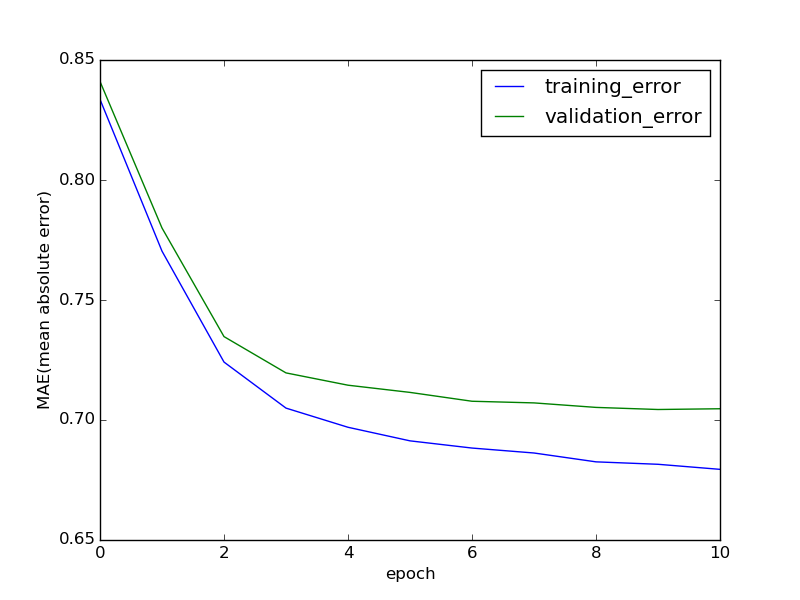
\includegraphics[width=0.5\linewidth]{training}
	\caption{An example learning process of 11 epochs(starting from epoch 0): 
	The estimator stopped learning at epoch 10 when validation error started 
	increasing.}
	\label{fig:trainnig}
\end{figure}

\subsection{Prediction accuracy}
The lowest testing error the estimator can achieve is 0.696.
This is better than the state-of-the-art testing error 0.740 achieved by 
collaborative filtering and category experts methods on this dataset 
\cite{hwang2016efficient}.
\autoref{tab:robust} shows that the estimator is also very robust against 
parameter changes.
.
\begin{table}[h]
	\centering
	\begin{tabularx}{\textwidth}{ |c|c|c|c|c|X| } \hline
		optimizer  & learning rate & dropout(keep probability) & layer size & 
		number of layers & 
		testing error \\ \hline
		SGD & 0.01 & 0.9 & 64 & 2 & 0.7009 \\ \hline
		SGD & 0.01 & 0.9 & 64 & 1 & 0.7129 \\ \hline
		SGD & 0.01 & 0.9 & 64 & 4 & 0.7151 \\ \hline
		SGD & 0.01 & 0.9 & 32 & 2 & 0.7120 \\ \hline
		SGD & 0.01 & 0.9 & 128 & 2 & 0.7177 \\ \hline
		SGD & 0.01 & 0.8 & 64 & 2 & 0.7007 \\ \hline
		SGD & 0.01 & 0.6 & 64 & 2 & 0.6956 \\ \hline
		SGD & 0.1 & 0.6 & 64 & 2 & 0.7019 \\ \hline
		SGD & 0.05 & 0.6 & 64 & 2 & 0.6985 \\ \hline
		Adagrad & 0.05 & 0.6 & 64 & 2 & 0.7143 \\ \hline
		Adagrad & 0.01 & 0.6 & 64 & 2 & 0.7109 \\ \hline
		Adagrad & 0.1 & 0.6 & 64 & 2 & 0.7114 \\ \hline
		Adagrad & 0.1 & 0.8 & 64 & 2 & 0.7058 \\ \hline
		Adagrad & 0.1 & 0.9 & 64 & 2 & 0.6925 \\ \hline
		Adagrad & 0.1 & 0.9 & 32 & 2 & 0.6965 \\ \hline
		Adagrad & 0.1 & 0.9 & 128 & 2 & 0.7026 \\ \hline
		Adagrad & 0.1 & 0.9 & 32 & 1 & 0.7032 \\ \hline
		Adagrad & 0.1 & 0.9 & 32 & 4 & 0.7008 \\ \hline
	\end{tabularx}
	\caption{High robustness of the estimator against parameter changes: 
	The estimator maintains testing errors in range [0.69, 0.72] for a wide 
	range of parameters.}
	\label{tab:robust}
\end{table}

\section{Strengths}

\subsection{Information mining: node-centered}
This technique takes a node-centered approach as the estimator extracts 
information about nodes from links.
In a social network, this leverages the fact that who a user contacts and what 
movies a user likes tell us what kind of person he is and helps us make 
recommendations for him.
It effectively learns complex and unobservable user attributes(node attributes) 
from simple and observable user activities(link attributes). 
\autoref{tab:nodesVSlinks} compares nodes and links with respect to their 
complexity and observability.
\begin{table}[h]
	\centering
	\begin{tabularx}{0.5\textwidth}{ |X|X|X| } \hline
		aspect  & node & link \\ \hline
		complexity & high & low \\ \hline
		observability & low & high \\ \hline
		example & user & activities \\ \hline
	\end{tabularx}
	\caption{A comparison of nodes and links with respect to their complexity 
		and attribute observability in a social network:
		Links tend to have low complexity and high observability while nodes 
		are the opposite.
		For example, it's easy to observe simple user activities like sending 
		messages to other users and give ratings to music,
		but it's hard to observe complex user attributes like personality, 
		style or taste in movies.}
	\label{tab:nodesVSlinks}
\end{table}

\subsection{Online learning}
The learning process is online (when the estimator learns for 1 epoch) so it 
naturally handles streaming graphs:
\begin{itemize}
	\item it can handle a new node by inserting a new vector into the mapping 
	table
	\item it doesn't need to handle new links as it uses every link once and 
	then discard the link
	\item it doesn't construct the graph or perform any complex graph 
	operations like neighbor nodes lookup
\end{itemize}

\section{Future work}
In order to generalize this node mapping technique to perform a wider range of 
prediction tasks related to making recommendations for users in a social 
network, we can consider to work on the following new features:
\begin{itemize}
	\item handle links connecting 2 nodes of the same type: e.g., given user A 
	and B, predict the amount of messages A send to B
	\item handle links with string attributes: e.g., given a text message from 
	user A to user B (a link from A to B with a string attribute), the 
	estimator should learn something about the users from the message content
	\item handle nodes with string attributes: e.g., given an article (a node 
	with a string attribute), the estimator should learn something about the 
	article from the article content
	\item handle links with logical implications: e.g., given a user has 
	written an article (a link from user to article with a write attribute), 
	the estimator should learn something about the user from this activity
\end{itemize}
We are open to collaborations so don't hesitate to contact us if you are 
interested in our work.

\section{Conclusions}
Node mapping is an effective technique to predict link attributes in a graph 
using a neural net model.
The estimator learns both to represent each node with a vector, and to predict 
the target link attribute using these vectors.
It achieves better rating prediction accuracy than the state-of-the-art 
collaborative filtering and category experts methods.
For recommendation tasks in social networks, this technique coincides with the 
idea of understanding complex users from their simple activities, and using 
that understanding to predict their future activities.

\bibliographystyle{acm}
\bibliography{references}

\end{document}
